\documentclass[a4paper,10pt]{article}

% For code example
\usepackage{listings}
\usepackage{xcolor}
\definecolor{codegreen}{rgb}{0,0.6,0}
\definecolor{codegray}{rgb}{0.5,0.5,0.5}
\definecolor{codepurple}{rgb}{0.58,0,0.82}
\definecolor{backcolour}{rgb}{0.95,0.95,0.92}
\lstdefinestyle{mystyle}{
    backgroundcolor=\color{backcolour},   
    commentstyle=\color{codegreen},
    keywordstyle=\color{magenta},
    numberstyle=\tiny\color{codegray},
    stringstyle=\color{codepurple},
    basicstyle=\ttfamily\footnotesize,
    breakatwhitespace=false,         
    breaklines=true,                 
    captionpos=b,                    
    keepspaces=true,                 
    numbers=left,                    
    numbersep=5pt,                  
    showspaces=false,                
    showstringspaces=false,
    showtabs=false,                  
    tabsize=2
}

\lstset{style=mystyle}

\usepackage{graphicx} % Required for inserting images
\usepackage[english]{babel}
%4 stackanchor  
\usepackage{stackengine}
% define nice looking boxes
\usepackage[many]{tcolorbox}

% a base set, that is then customised
\tcbset {
  base/.style={
    boxrule=0mm,
    leftrule=1mm,
    left=1.75mm,
    arc=0mm, 
    fonttitle=\bfseries, 
    colbacktitle=black!10!white, 
    coltitle=black, 
    toptitle=0.75mm, 
    bottomtitle=0.25mm,
    title={#1}
  }
}
\definecolor{brandblue}{rgb}{0.34, 0.7, 1}
\newtcolorbox{mainbox}[1]{
  colframe=brandblue, 
  base={#1}
}

\definecolor{orange}{rgb}{1, 0.55, 0.3}
\newtcolorbox{tbox}[1]{
  colframe=orange, 
  base={#1}
}

\definecolor{green}{rgb}{0.294, 0.729, 0.254}
\newtcolorbox{bembox}[1]{
  colframe=green, 
  base={#1}
}

\definecolor{red}{rgb}{0.99, 0.04, 0.99}
\newtcolorbox{tipbox}[1]{
  colframe=red, 
  base={#1}
}

\newtcolorbox{defbox}[1]{
  colframe=black!20!white,
  base={#1}
}
% Mathematical typesetting & symbols
\usepackage{amsthm, mathtools, amssymb} 
\usepackage{marvosym, wasysym}


\allowdisplaybreaks

% Tables
\usepackage{tabularx, multirow}
\usepackage{booktabs}
\renewcommand*{\arraystretch}{2}

% Make enumerations more compact
\usepackage{enumitem}
\setitemize{itemsep=0.5pt}
\setenumerate{itemsep=0.75pt}

% To include sketches & PDFs
\usepackage{graphicx}

% For hyperlinks
\usepackage{hyperref}
\hypersetup{
  colorlinks=true
}
% Math helper stuff
\def\limn{\lim_{n\to \infty}}
\def\limxo{\lim_{x\to 0}}
\def\limxi{\lim_{x\to\infty}}
\def\limxn{\lim_{x\to-\infty}}
\def\sumk{\sum_{k=1}^\infty}
\def\sumn{\sum_{n=0}^\infty}
\def\R{\mathbb{R}}
\def\dx{\text{ d}x}
\usepackage[utf8]{inputenc}

\title{SPCA Lecture Notes}
\author{Konstantin Lucny}
\date{HS 2023}

\begin{document}
\maketitle
\section{Vorlesung}
\subsection{Compile C Program}
\begin{itemize}
    \item \textbf{gcc}: C compiler
    \item \textbf{-o}: Specifies where the output should bw written to
    \item \textbf{touch}: Linux command to change time stamp of file
\end{itemize}
\subsection{Memory}
\begin{itemize}
    \item Memory is unbounded
    \item Memory is typed
    \item Performance \textbf{depends} on access pattern! Depending on acccess pattern the \textbf{stride} can differ. 
    \begin{figure}[htp]
    \centering
    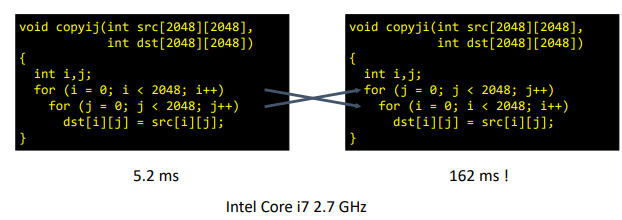
\includegraphics[width=13cm]{e1.png}
    \caption{Access pattern time difference}
    \label{fig:example}
\end{figure}
\end{itemize}
\subsection{Performance and Asymptotic Complexity}

\begin{itemize}
    \item Constant factors matter too -often more
    \item Even exact op count does not predict performance
\end{itemize}
\subsubsection{Example: matrix-matrix multiplication}
\begin{itemize}
    \item Fundamental operation in ML, graphics, etc...: $(...)\leftarrow(...)\times(...)$\\
    \begin{figure}[htp]
        \centering
        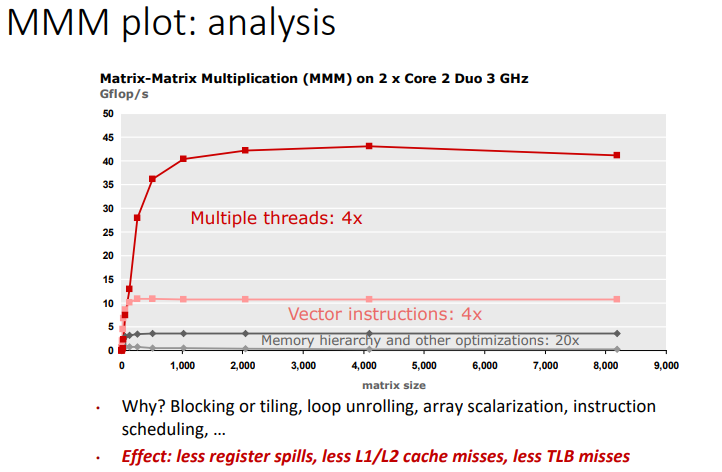
\includegraphics[width=11cm]{e2.png}
        \caption{Matrix Multiplication: analysis}
        \label{fig:enter-label}
    \end{figure}
\end{itemize}
\subsection{Role of "Standards"}
\begin{itemize}
    \item Language standards aim to \textbf{specify unambigously} what any program
in the language does when compiled and executed. (e.g. Java)
    \item The C standards should be viewed as rather different
    \begin{itemize}
        \item Behavior frequently describes as \textbf{implementation dependent}
    \end{itemize}
    \item \textbf{Implementation defined}: unspecified behavior where each implementation documents how the choice is made
    \begin{itemize}
        \item Compiler is allowed to do \textbf{anything}, so optimizes out the code completely (newer C-compilers)
        \item Compiler implements the \textbf{most natural mapping} to the target hardware and \textbf{documents} this. (older C-compilers)
    \end{itemize}
    \textbf{A program is a set of instructions to a compiler that tell it what assembly language to generate.}
\end{itemize}

\section{Vorlesung}
\subsection{C Overview}
\begin{itemize}
    \item \textbf{No} objects, classes, traits, features, methods, or interfaces
    \item \textbf{No} expections
    \item \textbf{No} automatic memory management
    \item \textbf{Def. Pointers}: direct access to memory adresses
\end{itemize}
C is about directly building and manipulating structures in main
memory!\\ 
\subsection{Hello World in C}
\begin{figure}[htp]
    \centering
    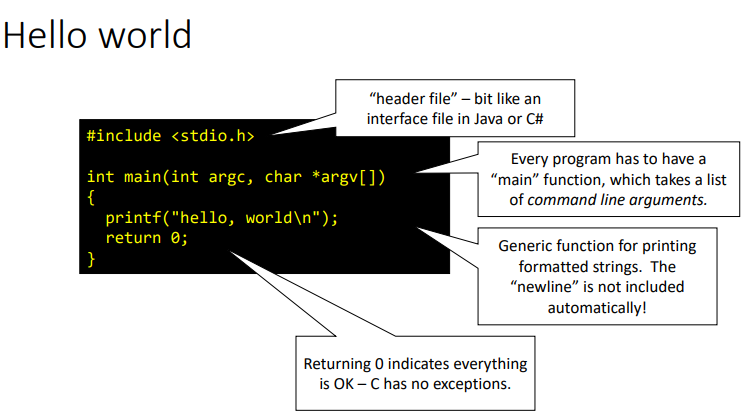
\includegraphics[width=1\linewidth]{e3.png}
    \caption{Hello World Program in C}
\end{figure}
\subsection{Workflow in C \& GNU gcc Toolchain}
\begin{figure}[htp]
    \centering
    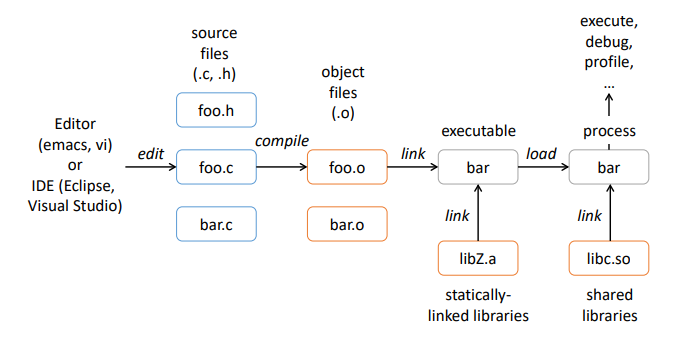
\includegraphics[width=1\linewidth]{e4.png}
    \caption{Workflow of C}
    \label{fig:enter-label}
\end{figure}
\begin{figure}[htp]
    \centering
    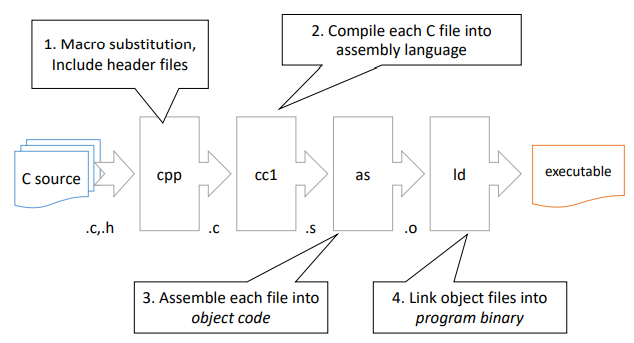
\includegraphics[width=1\linewidth]{e5.png}
    \caption{gcc Toolchain; cpp = macro pre-processor}
    \label{fig:enter-label}
\end{figure}
\begin{tipbox}
    {Info for gcc}
    \textit{gcc exampleC.c} (produces an executable file)
    \textit{-o difName} (changes Executable name)
    \textit{-c } (compiles the program and gives the object file as output, which is used to make libraries)
    To execute executable use: \textit{./exfileName}
\end{tipbox}

\subsection{Control flow statments}
Mostly same as Java

\textit{goto Label} (controversial, but sometimes very useful)
\pagebreak

\subsection{Functions in C}
\begin{figure}[h]
    \centering
    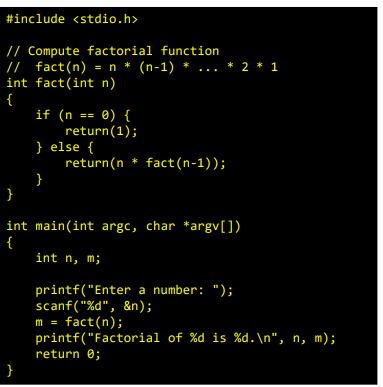
\includegraphics[width=0.75\linewidth]{e6.png}
    \caption{Introduction functions in C}
    \label{fig:enter-label}
\end{figure}

\subsection{Basic I/O}
\subsubsection{printf()}
\begin{figure}[h]
    \centering
    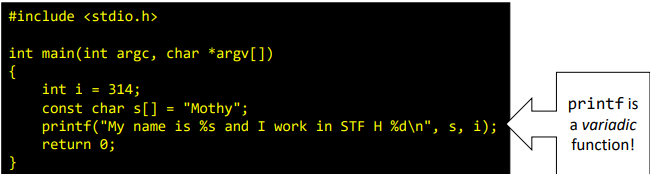
\includegraphics[width=1\linewidth]{e7.png}
    \caption{\textit{printf}}
    \label{fig:enter-label}
\end{figure}
\%d means number in decimal
\%s for argument s
\subsection{Summary control flow}
\begin{figure}[h!]
    \centering
    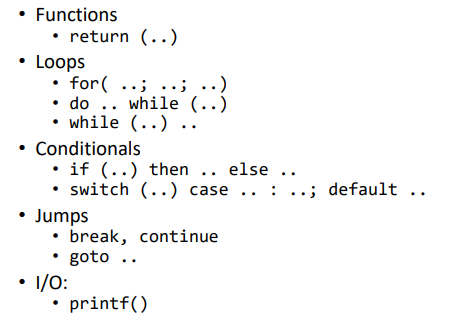
\includegraphics[width=0.7\linewidth]{e8.png}
    \caption{Summary control flow}
    \label{fig:enter-label}
\end{figure}

\pagebreak
\subsection{Declarations in C}
\begin{figure}[!h]
    \centering
    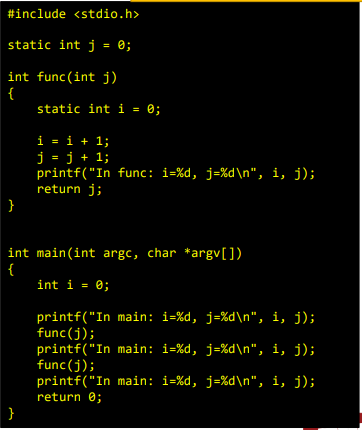
\includegraphics[width=0.75\linewidth]{e9.png}
    \caption{Declaration example}
    \label{fig:enter-label}
\end{figure}
\begin{tipbox}
    {Info declarations}
    \begin{itemize}
        \item Declaration in block: Scope is just the block \& \textit{static} $\rightarrow$ value \textbf{persist} between calls
        \item Declaration outside block: Scope is the entire program \& \textit{static} $\rightarrow$ scope limited to the file (\textbf{compilation unit})
    \end{itemize}
\end{tipbox}
\subsubsection{Integers and floats}
\begin{figure}[htp]
    \centering
    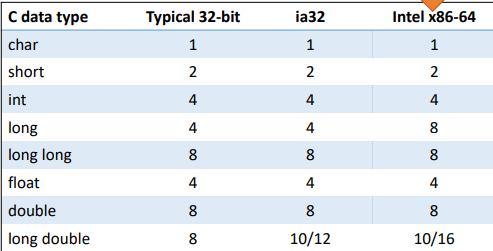
\includegraphics[width=1\linewidth]{e10.png}
    \caption{Types and sizes}
\end{figure}
\begin{tipbox}
    {}
    Integers are \textbf{signed} by default; however use \textit{signed} \& \textit{unsigned} for clarification
\end{tipbox}
\begin{figure}[h]
        \centering
        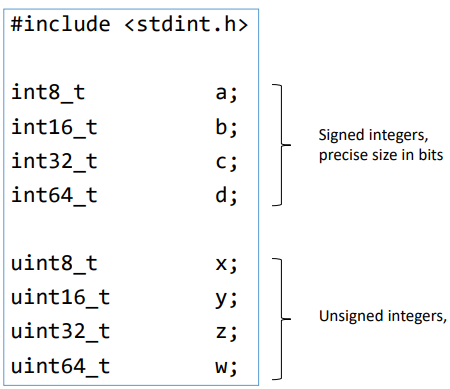
\includegraphics[width=0.7\linewidth]{e11.png}
        \caption{C99 extended integer types}
    \end{figure}
\pagebreak
\begin{tbox}
    {Rules for conversions}
    \begin{itemize}
        \item Implicit conversions between integer types
        \item implicit conversions between floating point types
        \item Explicit conversions between anything (casts)
    \end{itemize}
\end{tbox}
\subsubsection{Booleans}
\begin{itemize}
    \item False $\rightarrow$ zero
    \item True $\rightarrow$ anything non-zero
    \item Negations ("!") turns zero into non zero and vice-versa
\end{itemize}
\pagebreak
\begin{tipbox}
    {Important}
    Any statment in C is also an expression
\end{tipbox}
\begin{figure}[h]
    \centering
    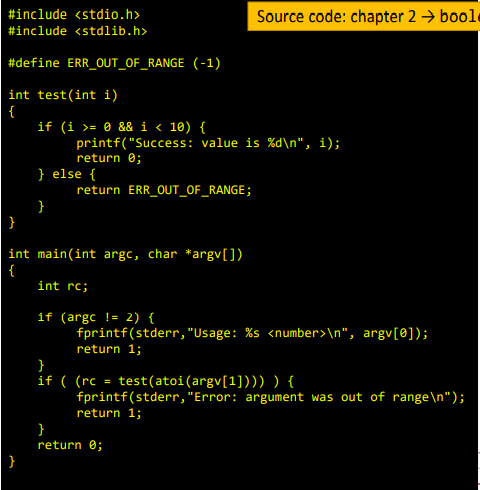
\includegraphics[width=0.7\linewidth]{e12.png}
    \caption{Example that any statement is an expression}
    \label{fig:enter-label}
\end{figure}
\subsubsection{void}
\begin{itemize}
    \item has \textbf{no} value
    \item used for
    \begin{itemize}
        \item Untyped pointers (to raw memory):“void *"
        \item Declaring functions with no return value (procedures)
    \end{itemize}
\end{itemize}
\pagebreak
\subsection{Operators in C}
\begin{figure}[h]
    \centering
    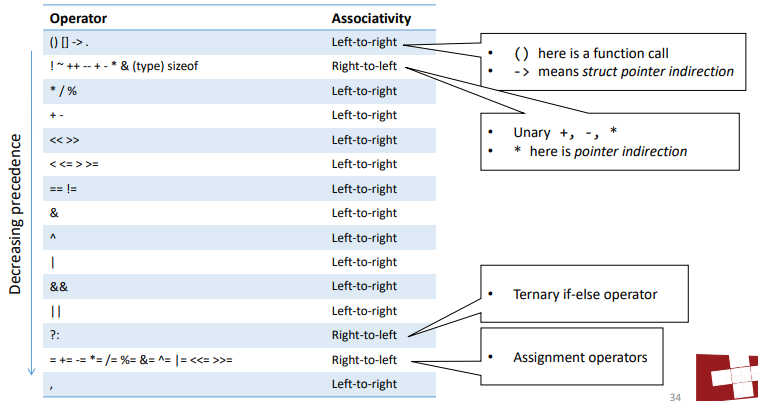
\includegraphics[width=1\linewidth]{e13.png}
    \caption{Operators in C}
    \label{fig:enter-label}
\end{figure}
\end{document}